\documentclass[tikz,border=2]{standalone}
\usetikzlibrary{shadows,arrows,shapes,positioning,calc,backgrounds,fit}
% Define the layers to draw the diagram
%
\begin{document}
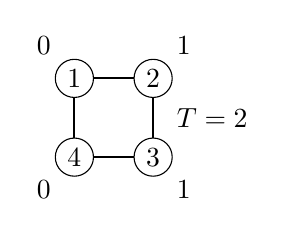
\begin{tikzpicture}
[node distance=1cm,
vertex/.style={shape=circle,draw=black,inner sep=2pt},
myedge/.style={thick}]
%%
\node (v1) [vertex,label=below left:$0$] at (0,0) {$4$};
\node (v2) [vertex,right of=v1,label=below right:$1$] {$3$};
\node (v3) [vertex,above of=v2,label=above right:$1$] {$2$};
\node (v4) [vertex,above of=v1,label=above left:$0$] {$1$};
\draw[myedge] (v1) -- (v2) -- (v3) -- (v4) -- (v1);
%% \draw[myedge,dashed] (v2) -- (v4);
\node at (1.75,.5) {$T=2$};
%%
\end{tikzpicture}
\end{document}
